\begin{figure}[H]
\begin{tabular}{@{}c@{}}
\begin{subfigure}[b]{0.5\textwidth}
\begin{center}
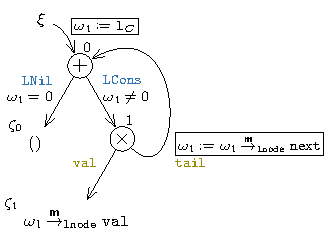
\includegraphics[scale=1.3]{chapters/figures/figValueTreeClistm.pdf}
\end{center}
\caption{\label{fig:valuetreeclistm}$\mathcal{V}(\lifted{list}{\mem{}}{lnode}{\cv{l}})$}
\end{subfigure}%
\begin{subfigure}[b]{0.5\textwidth}
\begin{center}
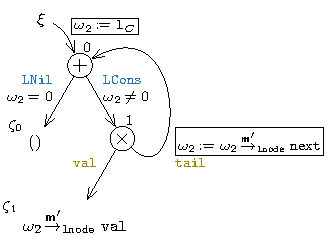
\includegraphics[scale=1.3]{chapters/figures/figValueTreeClistmdash.pdf}
\end{center}
\caption{\label{fig:valuetreeclistmdash}$\mathcal{V}(\lifted{list}{\mem{}'}{lnode}{\cv{l}})$}
\end{subfigure}%
\\
\begin{subfigure}[b]{\textwidth}
\begin{center}
% \begin{footnotesize}
\begin{tabular}{clll}
\toprule
{\bf Node Pair} & \multicolumn{3}{c}{\bf Invariants} \\
\toprule
$(\xi \!:\! \xi)$ & \multicolumn{3}{l}{$\circled{\small P} \  \lhs{}$ in \cref{eqn:cat3revisit}} \\
\midrule
\multirow{3}{*}{\makecell[c]{$(0 \!:\! 0)$ \\ $(1 \!:\! 1)$ }} & $\circled{\footnotesize I1} \  \vtse{1} = \vtse{2}$ & $\circled{\footnotesize I2} \  \vtse{1} \pointsTo{} \{ \mlrs{\cpc{4}}, \heapr \}$ & $\circled{\footnotesize I3} \  \vtse{2} \pointsTo{} \{ \mlrs{\cpc{4}}, \heapr \}$ \\
& $\circled{\footnotesize I4} \ \cv{p} \pointsTo{} \{ \mlrs{\cpc{4}} \}$ & $\circled{\footnotesize I5} \  \cv{l} \pointsTo{} \{ \mlrs{\cpc{4}} \}$ \\
& $\circled{\footnotesize I6} \ \mlrf{\cpc{4}} \pointsTo{} \{ \mlrs{\cpc{4}} \}$ & $\circled{\footnotesize I7} \  \mlrs{\cpc{4}} \pointsTo{} \{ \mlrs{\cpc{4}}, \heapr{} \}$ & $\circled{\footnotesize I8} \ \heapr{} \pointsTo{} \{ \mlrs{\cpc{4}}, \heapr{} \}$ \\
\midrule
$(\zeta_0 \!:\! \zeta_0)$ & \multicolumn{3}{l}{$\circled{\scriptsize E1} \  () = ()$} \\
\midrule
$(\zeta_1 \!:\! \zeta_1)$ & \multicolumn{3}{l}{$\circled{\scriptsize E2} \  \structPointer{\vtse{1}}{\mem{}}{lnode}{val} = \structPointer{\vtse{2}}{\mem{}'}{lnode}{val}$} \\
\bottomrule
\end{tabular}
% \end{footnotesize}
\end{center}
\caption{\label{fig:valuetreeinvs}Invariants table for bisimulation relation between \cref{fig:valuetreeclistm} and \cref{fig:valuetreeclistmdash}.}
\end{subfigure}
\end{tabular}
\caption{\label{fig:valuetreebisim}Value trees of \lifted{list}{\mem{}}{lnode}{\cv{l}} and \lifted{list}{\mem{}'}{lnode}{\cv{l}} along with
their associated node invariants at correlated node pairs.}
\end{figure}